\documentclass[a4paper,oneside,12pt]{report}
\setlength\textwidth{155mm}
\setlength\textheight{247mm}
\setlength\topmargin{-10mm}
\setlength\headheight{0mm}
\setlength\oddsidemargin{05mm}
\setlength\evensidemargin{05mm}
\let\openright=\clearpage


%% Vytváříme PDF/A-2u
\usepackage[a-2u]{pdfx}

%% Přepneme na českou sazbu a fonty Latin Modern
\usepackage[czech]{babel}
\usepackage{lmodern}
\usepackage[T1]{fontenc}
\usepackage{textcomp}

%% Použité kódování znaků: obvykle latin2, cp1250 nebo utf8:
\usepackage[utf8]{inputenc}

%%% Další užitečné balíčky (jsou součástí běžnýsrov.stribucí LaTeXu)
\usepackage{amsmath}        % rozšíření pro sazbu matematiky
\usepackage{amsfonts}       % matematické fonty
\usepackage{amsthm}         % sazba vět, definic apod.
\usepackage{bbding}         % balíček s nejrůznějšími symboly
			   										% (čtverečky, hvězdičky, tužtičky, nůžtičky, ...)
\usepackage{bm}             % tučné symboly (příkaz \bm)
\usepackage{graphicx}       % vkládání obrázků
\usepackage{fancyhdr}				% možnost slylizovat záhlaví
\usepackage{fancyvrb}       % vylepšené prostředí pro strojové písmo
\usepackage{indentfirst}    % zavede odsazení 1. odstavce kapitoly
\usepackage[nottoc]{tocbibind} % zajistí přidání seznamu literatury,
\usepackage{icomma}         % inteligetní čárka v matematickém módu
\usepackage{dcolumn}        % lepší zarovnání sloupců v tabulkách
\usepackage{booktabs}       % lepší vodorovné linky v tabulkách
\usepackage{paralist}       % lepší enumerate a itemize
\usepackage{caption}				%	popisky
\usepackage{dirtree}				% strom souborů
\usepackage{listings}				% vkládání kódu
\usepackage[bottom]{footmisc}  % poznámky pod čarou vespod
\usepackage{bibentry}
\usepackage{xurl}						% umožní url zalomit všude
\nobibliography*

\usepackage{color}
\usepackage{forest}					% na rodokmeny
\usepackage{natbib}
%\setbibentrystyle{author}

\definecolor{pblue}{rgb}{0.13,0.13,1}
\definecolor{pgreen}{rgb}{0,0.5,0}
\definecolor{pred}{rgb}{0.9,0,0}
\definecolor{pgrey}{rgb}{0.46,0.45,0.48}
\definecolor{apiblue}{HTML}{61AFFE}
\definecolor{apigreen}{HTML}{49CC90}
\definecolor{apicyan}{HTML}{50E3C2} % vím, že cyan je jiná barva % vím, že cyan je jiná barva
\definecolor{apired}{HTML}{F93E3E}
\definecolor{apiyellow}{HTML}{FCA130}
\renewcommand{\baselinestretch}{1.5}
%%% Údaje o práci

\def\NazevSkoly{Gymnázium, Praha 6, Arabská 14}
% Název oboru včetně počátečního 'Obor'.
\def\NazevOboru{Programování}

% Název práce v jazyce práce (přesně podle zadání)
\def\NazevPrace{Kontejnerizační systém pro školní server}

% Název práce v angličtině
\def\NazevPraceEN{Containerization system for school server}

% Název práce v němčině
\def\NazevPraceDE{Containerisierungssystem für Schulserver }

% Jméno autra
\def\AutorPrace{Havránek Kryštof, Vávra Vladimír, Litoš Josef 3.E }

% Rok odevzdání
\def\RokOdevzdani{2021}
% Měsíc odevzdání
\def\MesicOdevzdani{Duben}

% Vedoucí práce: Jméno a příjmení s~tituly
\def\Vedouci{Ing. Daniel Kahoun}

% Nepovinné poděkování (vedoucímu práce, konzultantovi, tomu, kdo
% zapůjčil software, literaturu apod.)
\def\Podekovani{%
\textbf{Poděkování}
}

% Abstrakt (doporučený rozsah cca 80-200 slov; nejedná se o zadání práce)
\def\Abstrakt{%
Cílem práce je vytvořit kontejnerizační systém pro operační systém GNU/Linux.
Ten by měl v jednoduchém a přehledném uživatelském prostředí umožnit žákům vytvořit si vlastný linuxový server.
Na kterém si poté mohou hostovat svoje aplikace, webové stránky, či videohry.
Systém by se měl postarat o to, aby zdroje serveru byly spravedlivě rozdělené mezi jednotlivé uživatele.
}

\def\AbstraktEN{%
Goal of the work is to create containerization system for GNU/Linux operating system.
With its help students should be able to create their own private server in a easy to use webUI.
On such server they will be able to host their applications, websites or video games.
System should also guarantee fair redistribution of server resources.
}
\def\AbstraktDE{%
Ziel des Werk ist ein Containerisierungssystem für das Betriebssystem GNU / Linux zu erstellen.
Es sollte den Schülern ihren eigenen Linux-Server in einer einfachen und übersichtlichen Benutzeroberfläche möglicher zu bilden.
Auf den Server können sie dann ihre Anwendungen, Websites oder Videospiele hosten, ich mag ein Brot.
Das System sollte sich zusichern, damit die Serverressourcen gerecht auf die individuellen Benutzer verteilt würden.
}
% 3 až 5 klíčových slov (doporučeno), každé uzavřeno ve složených závorkách
\def\KlicovaSlova{%
	{linux}, {lxd}, {lxc}, {kontejnery}, {nodejs}, {REST API}, {react js}
}
\def\KlicovaSlovaEN{%
	{linux}, {lxd}, {lxc}, {containers}, {nodejs}, {REST API}, {react js}
}

\def\KlicovaSlovaDE{%
	{linux}, {lxd}, {lxc}, {Schulprojekt}, {nodejs}, {REST API}, {react js}
}

%% Balíček hyperref, kterým jdou vyrábět klikací odkazy v PDF,
%% ale hlavně ho používáme k uložení metadat do PDF (včetně obsahu).
%% Většinu nastavítek přednastaví balíček pdfx.
\hypersetup{unicode}
\hypersetup{breaklinks=true}

%% Definice různých užitečných maker (viz popis uvnitř souboru)
%%% Tento soubor obsahuje definice různých užitečných maker a prostředí %%%
%%% Další makra připisujte sem, ať nepřekáží v ostatních souborech.     %%%

%%% Drobné úpravy stylu

% Tato makra přesvědčují mírně ošklivým trikem LaTeX, aby hlavičky kapitol
% sázel příčetněji a nevynechával nad nimi spoustu místa. Směle ignorujte.
\makeatletter
\def\@makechapterhead#1{
  {\parindent \z@ \raggedright \normalfont
   \Huge\bfseries \thechapter. #1
   \par\nobreak
   \vskip 20\p@
}}
\def\@makeschapterhead#1{
  {\parindent \z@ \raggedright \normalfont
   \Huge\bfseries #1
   \par\nobreak
   \vskip 20\p@
}}
\makeatother

% Toto makro definuje kapitolu, která není očíslovaná, ale je uvedena v obsahu.
\def\chapwithtoc#1{
\chapter*{#1}
\addcontentsline{toc}{chapter}{#1}
}

% Trochu volnější nastavení dělení slov, než je default.
\lefthyphenmin=2
\righthyphenmin=2

% Zapne černé "slimáky" na koncích řádků, které přetekly, abychom si
% jich lépe všimli.
\overfullrule=1mm

%%% Makra pro definice, věty, tvrzení, příklady, ... (vyžaduje baliček amsthm)

\theoremstyle{plain}
\newtheorem{veta}{Věta}
\newtheorem{lemma}[veta]{Lemma}
\newtheorem{tvrz}[veta]{Tvrzení}

\theoremstyle{plain}
\newtheorem{definice}{Definice}

\theoremstyle{remark}
\newtheorem*{dusl}{Důsledek}
\newtheorem*{pozn}{Poznámka}
\newtheorem*{prikl}{Příklad}

%%% Prostředí pro důkazy

\newenvironment{dukaz}{
  \par\medskip\noindent
  \textit{Důkaz}.
}{
\newline
\rightline{$\square$}  % nebo \SquareCastShadowBottomRight z balíčku bbding
}

%%% Prostředí pro sazbu kódu, případně vstupu/výstupu počítačových
%%% programů. (Vyžaduje balíček fancyvrb -- fancy verbatim.)

\DefineVerbatimEnvironment{code}{Verbatim}{fontsize=\small, frame=single}

%%% Prostor reálných, resp. přirozených čísel
\newcommand{\R}{\mathbb{R}}
\newcommand{\N}{\mathbb{N}}

%%% Užitečné operátory pro statistiku a pravděpodobnost
\DeclareMathOperator{\pr}{\textsf{P}}
\DeclareMathOperator{\E}{\textsf{E}\,}
\DeclareMathOperator{\var}{\textrm{var}}
\DeclareMathOperator{\sd}{\textrm{sd}}

%%% Příkaz pro transpozici vektoru/matice
\newcommand{\T}[1]{#1^\top}

%%% Vychytávky pro matematiku
\newcommand{\goto}{\rightarrow}
\newcommand{\gotop}{\stackrel{P}{\longrightarrow}}
\newcommand{\maon}[1]{o(n^{#1})}
\newcommand{\abs}[1]{\left|{#1}\right|}
\newcommand{\dint}{\int_0^\tau\!\!\int_0^\tau}
\newcommand{\isqr}[1]{\frac{1}{\sqrt{#1}}}

%%% Vychytávky pro tabulky
\newcommand{\pulrad}[1]{\raisebox{1.5ex}[0pt]{#1}}
\newcommand{\mc}[1]{\multicolumn{1}{c}{#1}}


%% Titulní strana a různé povinné informační strany
\fancypagestyle{plain}{
\fancyhf{}
\renewcommand{\headrulewidth}{0.4pt}
\renewcommand{\footrulewidth}{0.4pt}
\fancyhead[C]{}
\fancyhead[L]{Ročníková práce -- \NazevSkoly}
\fancyhead[R]{AvAvA}
\fancyfoot[L]{Vypracovali: \AutorPrace	(\NazevOboru)}
\fancyfoot[C]{}
\fancyfoot[R]{\thepage}
}



\begin{document}

%%% Titulní strana práce

\pagestyle{empty}
\hypersetup{pageanchor=false}

\begin{center}

{\LARGE\bfseries\NazevSkoly}

\vspace{-18mm}
\vfill

{\LARGE\NazevOboru}

\vfill

\centerline{\mbox{
\includegraphics[height=4cm]{../img/logo.png}}}

\vspace{-8mm}
\vfill

{\bf\Large ROČNÍKOÝ PROJEKT}

\vfill


\vspace{15mm}

{\LARGE\bfseries\NazevPrace}


\vfill


Vypracovali: \hfill \AutorPrace

Vedoucí práce: \hfill \Vedouci

\vspace{15mm}
\MesicOdevzdani \ \RokOdevzdani

\end{center}



\newpage
\hypersetup{pageanchor=true}
\pagestyle{plain}
\pagenumbering{roman}


\openright


\vspace*{\fill}


\noindent
Prohlašuji, že jsme jedinými autory tohoto projektu, všechny citace jsou
řádně označené a všechna použitá literatura a další zdroje jsou v práci uvedené.
Tímto dle zákona 121/2000 Sb. (tzv. Autorský zákon) ve znění pozdějších předpisů uděluji
bezúplatně škole Gymnázium, Praha 6, Arabská 14 oprávnění k výkonu práva na rozmnožování díla
(§ 13) a práva na sdělování díla veřejnosti (§ 18) na dobu časově neomezenou a bez omezení
územního rozsahu.


\vspace{1cm}

\noindent
V ........ dne ............
\hspace{4cm}
Podpisy autorů


\newpage
%
% %%% Poděkování
%
%\openright
%
\noindent
\Podekovani

\newpage


\openright

\vbox to 0.20\vsize{
\setlength\parindent{0mm}
\setlength\parskip{5mm}

Název práce:
\NazevPrace

Autoři:
\AutorPrace

% Vedoucí práce:
% \Vedouci, \KatedraVedouciho

Abstrakt:
\Abstrakt

Klíčová slova:
\KlicovaSlova

% Opakování v angličtině.

Title:
\NazevPraceEN

Authors:
\AutorPrace

Abstract:
\AbstraktEN

Key words:
\KlicovaSlovaEN


% Opakování v němčině.

Titlel:
\NazevPraceDE

Autoren:
\AutorPrace

Abstrakt:
\AbstraktDE

Schlüsselwörter:
\KlicovaSlovaDE

\vss}

\newpage

\openright



\tableofcontents


\newpage

\chapter*{Úvod}
\addcontentsline{toc}{chapter}{Úvod}

Cílem práce bylo postavit systém pro kontejnerizaci linuxového serveru, které by eventuálně mohl být nasazen na školním serveru.
Systém by spravedlivě rozdělil zdroje mezi jednotlivé žáky a poskytl jim již volný prostor, kde mohou testovat svoje aplikace.
Aktuálně totiž bylo problematické jen získat přístup na školní server.

O frontend práce se staral Vladimír, backend byl rozdělen mezi Kryštofa a Josefa.
Kde Josef se převážně věnoval propojení mezi backendem a lxd deamonem, zatímco Kryštof zpracoval integraci mySQL databáze.
Na spojení obou částí backendu a vytvoření route se podíleli oba členové týmu.

Vývoj probíhal na GitHubu -- \url{https://github.com/havrak/AvAvA}, kde je aplikace dostupná pod licencí GPLv3.
Projekt jsem testovali na vlastní VPS.




\pagenumbering{arabic}
\setcounter{page}{1}

\chapter{Architektura}

\begin{figure}[h]
	\centering
	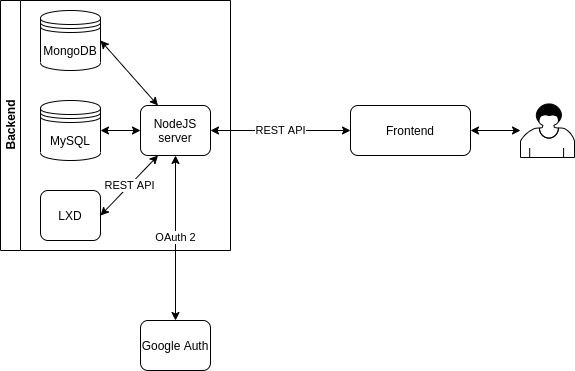
\includegraphics[height=9.5cm]{../img/architecture.png}
	\caption[Strukura projektu, vlastní tvorba]{Struktura projektu}
	\label{fig:architecture}
\end{figure}

Jádro práce stojí na lxd, což je kontejnerizační systém zabudovaný přímo do linuxového kernelu.
Jedná se tak o nejvíce efektivní řešení, protože jednotlivé kontejnery mohou sdílet společný kernel.
Jsou tak menší a rychlejší, než kdyby se jednalo o VPS.
Backend s lxd komunikuje prostřednictvím REST API, které lxd přímo podporuje.

Samotný backend je napsán v nodejs a ke svému fungování využívá dva databázové systémy.
Většinu informací ukládá do mySQL databáze, kvůli komplikacím s LXD byla později zavedena mongoDB.

Frontend je psán v ReactJS a s backendem komunikuje prostřednictvím vlastního REST API (jehož podrobná specifikace je uvedena v dokumentaci).
Na frontendu může uživatel v pohodlném prostředí vytvářet nové kontejnery, projekty, či získat informace o jejich aktuálním stavu a mnohé další.


\section{Specifikace vlastního API}


\subsubsection{\color{apiblue}{GET -- /api/combinedData}}

Routa GET /api/combinedData vrací objekt UserData.
Odpověď obsahuje informace o uživateli, informace potřebné k vytvoření nového kontejneru (Dostupné šablony a aplikace, které je možno nainstalovat.)
Mimo to je v odpovědi objekt UserProjects, který v sobě má uložené limity uživatele a informace o všech jeho projektech.
Jedná se o jeden z prvních požadavků co frontend zavolá.

\subsubsection{\color{apiblue}{POST -- /api/instances}}

Routa POST /api/instances umožňuje uživateli vytvořit nový kontejner.
Překročil li uživatel aktuální maximální limity, či vytvoření kontejneru selhalo vrátí se uživateli chybová hláška s kódem 400.
Kontejner se pochopitelně smaže z databáze, kam je nutné ho provní uložit.

Požadavek také umožňuje nechat na kontejner nainstalovat aplikace, selže li jejich instalace uživatel se o tom nedozví.
Kontejner se však nesmaže.

Vytvoří li se dobře kontejner vrátí se uživateli Container objekt obsahující informace o právě vytvořeném kontejneru.
Na backendu se zároveň vygeneruje nový konfigurační soubory proxy (viz. Backend$\Rightarrow$ Networking $\Rightarrow$ Proxy).


\subsubsection{\color{apiblue}{GET -- /api/instances/createInstanceConfigData}}

Routa GET /api/instances/createInstanceConfigData slouží vrací objekt createInstanceConfigData.
Je volána vždy před vytvořením nového kontejneru, aby uživatel měl na výběr mezi aktuální nabídkou šablon a aplikací, které je možno nainstalovat.

\subsubsection{\color{apiblue}{GET -- /api/instances/\{id\}}}

Routa GET /api/instances/\{id\} vrací objekt Container.
V něm jsou uložené informace o dotazovaném kontejneru, jako jsou jeho limity, či aktuální stav.
Jak bylo zmíněno v autorizaci, uživatel se může zeptat pouze na kontejnery, které vlastní, či je na nich uveden jako spolupracovník.

\subsubsection{\color{apicyan}{PATCH -- /api/instances/\{id\}}}

Routa PATCH /api/instances/\{id\} slouží k změně limitů kontejnerů.
Aktuálně není změna limitů na backendu implementována.
Po změně limitů by se měla vrátit objekt Container s novými limity a všechny záznamy v containersResourcesLog by byly vymazány.
Změna limitů jde provádět pouze na vypnutém kontejneru, o to by se routa postarala.

\subsubsection{\color{apired}{DELETE -- /api/instances/\{id\}}}

Routa DELETE /api/instances/\{id\} slouží k smazání vybraného kontejneru.
Operace nejde nijak revertnou, neudělal li si uživatel backup.
Kontejner se jednoduše smaže z databáze a z lxd systému.

\subsubsection{\color{apiblue}{GET -- /api/instances/\{id\}/stateWithHistory}}

Routa GET /api/instances/\{id\}/stateWithHistory vrací pole objektů ContainerStateWithHistory.
V něm je uloženo id kontejneru a logy stavu kontejneru (prostřednictvím ContainerResourceState).
S aktuální konfigurací je stav zaznamenává co deset minut dvě hodiny nejstarší stav byl zaznamenám před 2 hodinami.

V objektech jsou vyplněna pouze pole, které jsou uloženy v databázi, tedy informace o stavu ram, cpu, počtu procesů, rychlosti uploadu, rychlosti downloadu a limity.
Výjimku představuje poslední ContainerResourceState v poli, kde je uložen aktuální stav, který se získá přes volání do lxd.

\subsubsection{\color{apiblue}{GET -- /api/instances/\{id\}/console}}

Routa GET /api/instances/\{id\}/console slouží realizaci konzole ve webovém prostředí.
Na serveru se vytvoří websocket s konzolí a přihlašovací údaje na něj se zašlou uživateli.

\subsubsection{\color{apiblue}{GET -- /api/instances/\{id\}/snapshots}}

Routa GET /api/instances/\{id\}/snapshots má sloužit k získání snapshotů kontejnerů.
V aktuální verzi není routa implementována, obnovení snapshotu se totiž objevilo jako velmi problematické.
Podobně jako u backupu se i u snapshotu musí řešit limity, zde jsou však uložené ve snapshotu.
Uživatel by měl možnost vybrat si jaký snapshots chce obnovit a jaké jeho limity se mají dodržet.
Logika obnovení byla příliš složitá a její realizace se nestihla včas udělat.


\subsubsection{\color{apigreen}{POST -- /api/instances/\{id\}/snapshots}}

Routa POST /api/instances/\{id\}/snapshots by měla vyvolat vytvoření snapshotu kontejneru.
Stejně jako další routy týkající se logiky snapshotů ani tato nebyla implementována.

\subsubsection{\color{apired}{DELETE -- /api/instances/\{id\}/snapshots/\{snapshotsid\}}}

Routa DELETE /api/instances/\{id\}/restore/\{snapshotsid\} by měla smazat snapshots
Stejně jako další routy týkající se logiky snapshotů ani tato nebyla implementována.

\subsubsection{\color{apicyan}{PATCH -- /api/instances/\{id\}/restore/\{snapshotsid\}}}

Routa PATCH /api/instances/\{id\}/restore/\{snapshotsid\}

\subsubsection{\color{apiblue}{GET -- /api/instances/\{id\}/export}}

Routa GET /api/instances/\{id\}/export slouží k exportování backupu.
Po jejím zavolání se na serveru vytvoří backup kontejneru a přes data stream se pošle uživateli.
Aktuálně je kompresován ve formátu .tar.gz.

\subsubsection{\color{apiyellow}{PUT -- /api/instances/import}}

Routa PUT /api/instances/import má sloužit k importu backupu kontejneru.
V aktuální verzi není routa implementována, je totiž problematické zjistit stav limitů z backup.
Routa by měla kontejner deplounout v sandboxu a zjistit si jeho limity.
Poté ověřit zda uživatel má volné zdroje na jeho vytvoření, pokud ano kontejner by se vytvořil a zapsal do databáze.


\subsubsection{\color{apicyan}{PATCH -- /api/instances/\{id\}/start}}

Routa PATCH  /api/instances/\{id\}/start slouží k nastartování kontejneru.
Pokud se kontejner nastartuje jeho aktuální stav se uloží do databáze a vygeneruje se objekt Container.
Ten se pošle jako odpověď na požadavek.

\subsubsection{\color{apicyan}{PATCH -- /api/instances/\{id\}/stop}}

Routa PATCH  /api/instances/\{id\}/stop slouží k stopnutí kontejneru.
Před zastavením se uloží jeho stav, se změněnými hodnotami (status bude stopped, využití ram nula, atd.), do mongoDB.
Není totiž možné získat stav kontejneru je li stopnutý.
Pokud se kontejner pozastaví jeho aktuální stav se uloží do mySQL databáze a vygeneruje se objekt Container.
Ten se pošle jako odpověď na požadavek.


\subsubsection{\color{apicyan}{PATCH -- /api/instances/\{id\}/freeze}}

Routa PATCH  /api/instances/\{id\}/freeze slouží k zmražení kontejneru.
Pokud se kontejner zmrazí jeho aktuální stav se uloží do databáze a vygeneruje se objekt Container.
Ten se pošle jako odpověď na požadavek.


\subsubsection{\color{apicyan}{PATCH -- /api/instances/\{id\}/unfreeze}}

Routa PATCH  /api/instances/\{id\}/unfreeze slouží k rozmražení kontejneru.
Pokud se kontejner rozmrazí jeho aktuální stav se uloží do databáze a vygeneruje se objekt Container.
Ten se pošle jako odpověď na požadavek.


\subsubsection{\color{apiblue}{GET -- /api/projects}}

Routa GET /api/projects vrací objekt UserProjects.
V něm jsou uložené limity uživatele a pole objektů Project s inforamcemi o jeho projektech a kontejnerech v nich.

\subsubsection{\color{apigreen}{POST -- /api/projects}}

Routa POST /api/projects slouží k vytvoření nové projektu.
Prvně se zkontroluje, zda uživatel má místo na jeho vytvoření.
Pokud ano, tak se vygeneruje JSON, jenž se odešle do lxd.
U projektu lze limitovat pouze využití ram a využití disku.
Oba limity se v praxi ukázali problematické a v projektu s nastavenými limity nešel vytvořit žádný kontejner.

Systém podporuje projekt s nulovými (null, ne nula) limity, aktuálně je však nejde mixovat.

Odpovědí na request je objekt Projekt, který se vygeneruje je li vytvoření projektu úspěšné.

\subsubsection{\color{apiblue}{GET -- /api/projects/stateWithHistory}}

Routa GET /api/projects/stateWithHistory vrací objekt UserStateWithHistory.
V něm je uložená historie všech projektů uživatele, které obsahuje historii jeho všech kontejnerů.

\subsubsection{\color{apiblue}{GET -- /api/projects/\{id\}}}

Routa GET /api/projects/\{id\} vrací objekt Project s informacemi o projektu.
Ten si mimo jiné pamatuje limity, název, spolupracovníky a pole Container objektů.

\subsubsection{\color{apicyan}{PATCH -- /api/projects/\{id\}}}

Routa PATCH /api/projects/\{id\} slouží k úpravě limitů projektu.
V aktuální verzi je možno limity pouze zvýšit a projekt přejmenovat.
Je li projekt přejmenován vygeneruje se nová konfigurace proxy.
Odpovědí na request je objekt Project s novými limity projektu.

\subsubsection{\color{apired}{DELETE -- /api/projects/\{id\}}}

Routa DELETE /api/projects/\{id\} slouží k smazání projektu.
Stejně jako  smazání kontejneru ani smazání projektu nejde vrátit zpět.
Metoda prvně smaže veškeré kontejnery nacházející se v projektu a poté projekt samotný.

\subsubsection{\color{apiblue}{GET -- /api/projects/\{id\}/stateWithHistory}}

Routa GET /api/projects/\{id\}/stateWithHistory vrací objekt ProjectStateWithHistory.
V něm je uložená historie všech kontejnerů projektu, která využívá stejnou metodu jako GET /api/instances/stateWithHistory.

\subsubsection{\color{apiblue}{GET -- /api/user}}

Routa GET /api/user vrací objekt User.
Jedná se o právě přihlášeného uživatele.

\subsubsection{\color{apiblue}{GET -- /api/logout}}

Routa GET /api/logout uživatel odhlásí ze systému.


\section{Autentifikace}

\begin{figure}[h]
	\centering
	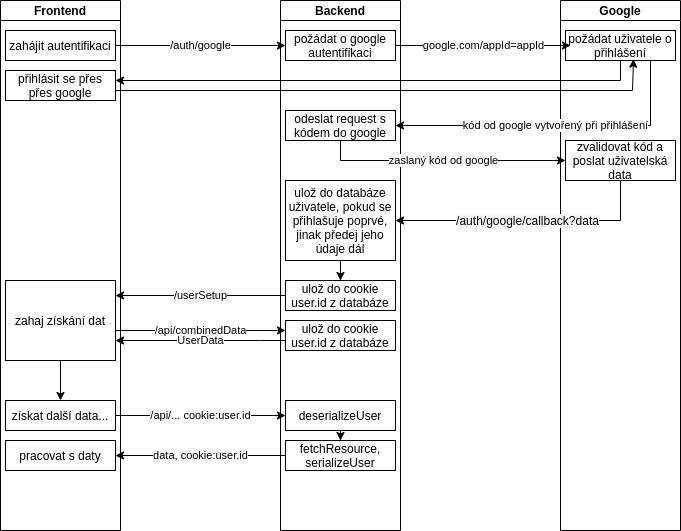
\includegraphics[height=9.5cm]{../img/authentication.png}
	\caption[Autentifikace přes googleAuth 2.0, vlastní tvorba]{Autentifikace přes googleAuth 2.0}
	\label{fig:architecture}
\end{figure}

Za způsob autentifikace uživatelů byl zvolen Google Auth, jelikož všichni studenti gymnázia Arabská mají svůj vlastní školní Google účet. Díky tomu si každý student bude moci vytvořit vlastní server bez nutnosti registrace.

Pro zprovoznění autentifikace je nejprve nutné si v Google Console vytvořit nový projekt.
Aktuálně je tento projekt hoštěn na studentském Google účtu \url{vladimir.vavra@student.gyarab.cz.} % easyest way to force linebreak
Je nastavené, že pouze uživatelé v rámci domény .gyarab se mohou do systému přihlásit.
Poté, co se nastaví všechna potřebná data je vygenerován clientId a clientSecret, což jsou kódy, pomocí nichž se bude AvAvA autorizovat

\subsection{Princip fungování}

Na obrázku výše můžete vidět průběh autentifikačního procesu.
Nejprve uživatel musí autentifikaci zahájit, což udělá pokusem o získání nějakého chráněného obsahu.
Po odeslání žádosti z klienta na backend přesměruje uživatele na přihlašovací stránku Google.
V případě, že se student přihlásí poprvé, musí odsouhlasit, že povoluje programu využívat některé služby.
Při dalších návštěvách se už jen přihlásí.

Tím je proces autentifikace hotov a začíná proces autorizace programu u Googlu.
AvAvA tedy bude Google žádat, aby jí předal data o uživateli, která potřebuje.
To dělá v obdélníku “odelsat request s kódem do google”.
Pokud google vyhoví, zavolá callback, který mu byl nastaven při vytváření projektu v Google Console a odešle na něj chtěná data.
V případě, že se uživatel přihlásil poprvé, je o něm uložen záznam do databáze, se kterým poté backend bude párovat kontejnery a projekty.
Následně je vytvořena session mezi frontendem a backendem. Každá zpráva odteď bude v hlavičce obsahovat cookie soubor s ID uživatele.

Po získání dat je uživatel přihlášen a může systém používat. Při odhlášení je session ukončena a už se dále user ID neposílá.

\subsection{Implementace}


Při implementaci byla hlavním zdrojem informací videa, ze kterých jsme získali část kódu\footnote{\bibentry{googleAuth}}.
Jelikož celý proces autentifikace probíhal na backendu, je uživatel odkázán na frontendovou cestu /userSetup. To je signál, že se uživatel přihlásil a frontend tedy pošle žádost na /api/combinedData.

Pro implementaci tohoto procesu na backendu bylo využito knihovny passport.js, která celý proces usnadňuje. Jediné, co je potřeba udělat je implementovat metody serializeUser a deserializeUser, které se budou volat po pořadě při zapisování ID do sessioncookie a při získávání uživatele z databáze za pomoci ID získané ze sessioncookie.

Je také nutné zapsat kód, který se zavolá hned po přihlášení, tedy uložení do databáze - passport.use(...) a předat passportu clientId a secretId.

Pro zjištění, zda je uživatel přihlášen je možné na kterékoliv z request objektů získat property req.user, ve které bude uložen výsledek posledního volání metody deserializeUser. V případě, že žádný uživatel není přihlášen, jeho hodnota je null. K tomuto účelu slouží metoda isLoggedIn


\subsection{Autorizace}

Pro každý request do API se zkontroluje, zda je uživatel přihlášen.
Není li přihlášen vrátí se mu kód 401 se zprávou, že není autentifikován.
Jelikož metody počítají s emailem, který do requestů přidává googleAuth, tak není možné vykonat pro nepřihlášeného uživatele ani get requesty.
Navíc není, žádoucí aby uživatel viděl stav ostatních uživatelů.

Routy, které obsahují id kontejneru, či projektu si ověřují zda je odesílatel requestu má právo upravovat kontejneru.
U kontejneru, k tomu slouží metoda userSQL.doesUser\linebreak OwnGivenContainer(email,id).
Ta interně zavolá metod userSQL.doesUserOwnGiven\linebreak Project(email, id), poté co zjistí id projektu z databáze.
Činý tak jelikož pokud má uživatel právo na projektu, má zároveň právo na jeho kontejneru.

V aktuálním podobě se ověřuje zda je uživatel uveden buďto jako vlastník, nebo spolupracovník na projektu.
Eventuálně by měl superadmin a admin mýt právo cizí kontejnery do určité míry ovlivňovat.
Konkrétně admin na ně pouze nahlížet a superadmin s nimi volně zacházet a měnit je.

Ověření metodou userSQL.doesUserOwnGivenProject(email, id) používá také routa /api/instances\#POST.
Zde je třeba ověřit zda uživatel vlastní projekt, do kterého se snaží vytvořit nový kontejner.


\chapter{Frontend}

Základem pro frontend se stal dashboard template\footnote{viz. \bibentry{templates}}.
 Požadavky aplikace ovšem tento template ani zdaleka nedokázal splnit. Jedinými částmi, které tedy přebrány je layout aplikace (soubor User), design Sidebaru a Navbaru, způsob strukturování složek včetně jejich mobilních verzí.
 I tyto části ovšem musely být modifikovány, aby vyhovovaly všem nárokům aplikace.
 Zároveň také z templatu zůstaly scss soubory.
 Ty jsou ovšem využívány některými komponentami, takže zatím soubory nebyly z projektu vymazány.

 Kód byl napsaný v Javascriptu, konkrétně ReactJS a preprocessoru SASS. Velice důležité jsou i knihovny react-bootstrap a material-ui, pomocí nichž byla napsána většina komponent.

\section{Struktura souborů}

Následující sekce popisuje strukturu souborů clienta.

\begin{figure}[h]
	\dirtree{%
	.1 client.
	.2 node\_modules.
	.2 public.
	.2 src.
	.3 actions.
	.3 api.
	.3 assets.
	.3 components.
	.3 layouts.
	.3 reducers.
	.3 service.
	.3 views.
	.3 App.js.
	.3 index.js.
	.3 logo.svg.
	.3 routes.js.
	.3 setupProxy.js.
	}
	\caption[Struktura souborů frontendu, vlastní tvorba]{Struktura souborů frontend}
	\label{fig:frontendStructure}
\end{figure}


%public
\subsubsection{Public}
\begin{figure}[h]
	\dirtree{%
	.1 client.
	.2 public.
	.3 favicon.ico.
	.3 index.html.
	}
	\caption[Struktura souborů frontendu, vlastní tvorba]{Struktura souborů frontend}
	\label{fig:frontendStructure}
\end{figure}
Ve složce public se nachází pouze jeden HTML soubor s root divem, do kterého React zapisuje.
Favicon je poté LXD ikona, která se objeví jako ikona karty prohlížeče.

Soubory .eslintcache, package=lock.json jsou automaticky generované a nejsou tedy důležité.
Soubor gulpfile.js připne k HTML a CSS souborům hlavičku, kterou vyžaduje licence templatu.
Soubor jsconfig.json poté dovolí importovat soubory pomocí absolutních cest vzhledem k src složce, což činí práci s importy mnohem pohodlnější

\subsubsection{Src}
\begin{figure}[h]
	\dirtree{%
	.1 client.
	.2 src.
	.3 actions.
	.3 api.
	.3 assets.
	.3 components.
	.3 layouts.
	.3 redurcers.
	.3 service.
	.3 views.
	.3 App.js.
	.3 inedex.js.
	.3 logo.svg.
	.3 routes.js.
	.3 setupProxy.js.
	}
	\caption[Struktura souborů frontendu, vlastní tvorba -- src]{Struktura souborů frontend -- src}
	\label{fig:frontendStructureSrc}
\end{figure}
Zdaleka nejdůležitější je ovšem src složka, která obsahuje samotný kód.
Půjdeme-li popořadě, tak první složkou je actions, kde se nacházejí akce manipulující s Redux storem (viz kapitola 2..).
S ním také manipulují reducery ve složce redurcers.


\newpage
\subsubsection{Api}


\begin{figure}[h]
	\dirtree{%
	.1 client.
	.2 src.
	.3 api.
	.4 api.
	.4 model.
	.4 ApiClient.js.
	.4 index.js.
	.4 WebSockets.js.
	}
	\caption[Struktura souborů frontendu -- api, vlastní tvorba]{Struktura souborů frontend -- api}
	\label{fig:frontendStructureApi}
\end{figure}
Ve složce api se nachází kód na získání a odesílání dat na backend (viz kapitola 2.2).

\subsubsection{Assets}

\begin{figure}[h]
	\dirtree{%
	.1 client.
	.2 src.
	.3 assets.
	.4 css.
	.4 fonts.
	.4 img.
	.4 scss.
	.5 custom.
	.5 lbd.
	.5 lbdr.
	}
	\caption[Struktura souborů frontendu -- assets , vlastní tvorba]{Struktura souborů frontend -- assets}
	\label{fig:frontendStructureAssets}
\end{figure}
Ve složce assets se nachází vše, co se týká stylů, obrázků a fontů potřebných pro projekt.
Kód napsaný v assets/scss se díky preprocessoru zkompiluje do css souborů do složky assets/css, které se poté odesílají spolu s HTML souborem.
Většina stylů byla zachována z templatu, jelikož jsou styly vcelku použitelné i na požadavky projektu. Například díky nim funguje responzivní navigace.

V některých případech bylo ovšem nutné napsat vlastní styly.
Ty jsou uloženy ve složce assets/scss/custom.
Do souboru light-bootstrap-dashboard je poté přidán import každého z custom souborů.

\newpage
\subsubsection{Components}

\begin{figure}[h]
	\dirtree{%
	.1 client.
	.2 src.
	.3 components.
	.4 Cards.
	.4 Dialogs.
	.4 Footer.
	.4 Form.
	.4 Icons.
	.4 Navbar.
	.4 RouteComponents.
	.4 Sidebar.
	.4 Tables.
	.4 Terminal.
	.4 ProjtecedRoute.js.
	.4 UserSetup.js.
	}
	\caption[Struktura souborů -- components, vlastní tvorba]{Struktura souborů -- components}
	\label{fig:frontendStructureComponentes}
\end{figure}

Složka components obsahuje znovupoužitelné komponenty, ze kterých se poté skládají jednotlivé stránky.
Na ní přímo navazuje složka views, v níž se nachází kód, který jednotlivé komponenty spojuje do stránek.
Když tedy uživatel zadá do URL baru cestu, zobrazí se mu právě jedna stránka složená z několik komponent.
Tyto stránky jsou poté obaleny ještě do tzv. layoutů nacházejících se ve složce layout.
Stránky jsou v nich spojeny s navigacemi a zápatím.
Momentálně existuje pouze jeden layout a to layout pro uživatele (User.js).
V budoucnu je ovšem plánováno rozšířit také projekt pro administrátorský přístup, layouty tedy přibydou.



\subsubsection{Service}


Ve složce service se nacházejí služby, které mohou využívat jakékoliv další služby.
Jedná se o různé druhy výpočtů, např. převádění jednotek, počítání stavů grafů atd...

Soubor index.js je nejvyšším souborem, který do root divu v HTML vloží celý frontend.
Zároveň obsahuje kód pro integraci reduxu.
Soubor App.js obsahuje komponent, který seskupuje všechny layouty a dovoluje a podílí se na navigaci na frontendu (viz kapitola 2.4).
Stejně tak si v kapitole probereme i soubor routes.js.

\newpage
\subsubsection{View}

\begin{figure}[h]
	\dirtree{%
	.1 client.
	.2 src.
	.3 views.
	.4 Containers.
	.5 Console.js.
	.5 Container.js.
	.5 Info.js.
	.5 Snapshots.js.
	.5 StateHistory.js.
	.4 Other.
	.4 Projects.
	.5 Container.js.
	.5 Info.js.
	.5 Project.js.
	.4 User.
	.5 Dashboard.js.
	.5 Project.js.
	.6 UserProfiel.js.
	}
	\caption[Struktura souborů -- view, vlastní tvorba]{Struktura souborů -- view}
	\label{fig:frontendStructureView}
\end{figure}

Ve složce views sídlí jednotlivé stránky.
Ty jsou v ní dále rozděleny podle toho, do jaké kategorie spadají.
Zde jsou vidět všechny tři kategorie.
Ve složce Other se poté nacházejí stránky z templatu pro případ, kdy by bylo možné někdy použít některé z template komponentů.

\newpage
\section{API}

Veškerý kód, který má něco společného s komunikaci s backendem či jinými externími zdroji sídlí ve složce api.
Obsah této složky kromě WebSockets.js je generován pomocí programu swagger-codegen v již zmíněném Swagger editoru.

Ve složce api/api se poté nachází soubor, kde jsou vygenerované metody odpovídající cestám na REST API, těmto metodám stačí předat specifikované parametry a na server se odešlou požadovaná data.
Po získání odpovědi je zavolán předaný callback.

Swagger codegen vygeneroval soubory, které jako API klienta používají knihovnu superagent.
Jeho chování je specifikováno pomocí vygenerovaného souboru ApiClient.
Vygenerovaný kód ovšem nestačí, např. pokud by vrácená odpověď byla 401, tak bylo nutné do souboru přidat příkaz na spuštění autentifikace.

Ve složce models se nachází soubory odpovídající objektům z Open API specifikace.
Na frontendu je ovšem vůbec nevyužívám, slouží tedy pouze samotnému fungování API.

Vše je poté přehledně dostupné v souboru index.js, ze kterého jsou exportovány všechny objekty z model složky a cesty z api/api/DefaultAPI.js

Posledním souborem je WebSockets.js, ve kterém se nachází metody vytvářející WebSocket spojení na backend.
Momentálně se WebSockety využívají pouze pro vytvoření spojení pro terminál do kontejnerů, ale v budoucnosti je očekávané, že se jejich využití rozšíří.
V případě, že bude spolu na jednom projektu spolupracovat více uživatelů, bude nutné pro vytvoření real-time systému updatovat změny pomocí duplexního spojení, kterým je právě WebSocket.

Jelikož při developmentu nejsou backend a frontend na jednom portu, dochází ke CORS erroru.
Na jeho vyřešení byla implementována http proxy (soubor setupProxy.js), která veškeré specifikované requesty přesouvá na port 5000 se stejnou adresou.

\section{Redux}

Redux je framework, který dovoluje různým React komponentům sdílet stav pomocí tzv. Redux store.
V případě, že nějaký komponent potřebuje přistoupit k nějaké části storu, tak se napíše metoda mapStateToProps a jednotlivé proměnné jsou poté předány jako properties jednotlivým komponentám.
V případě, že dojde ke změně redux storu, dojde k překreslení daného komponentu.


Základní chování Redux storu je, že se vynuluje při načtení stránky.
Z tohoto důvodu se store ukládá do localstorage při každé jeho změně.
Při načtení stránky se poté z localstorage načte zpět.
O inicializaci a chování stavu se stará soubor index.js v src složce.

\begin{figure}[h]
	\centering
	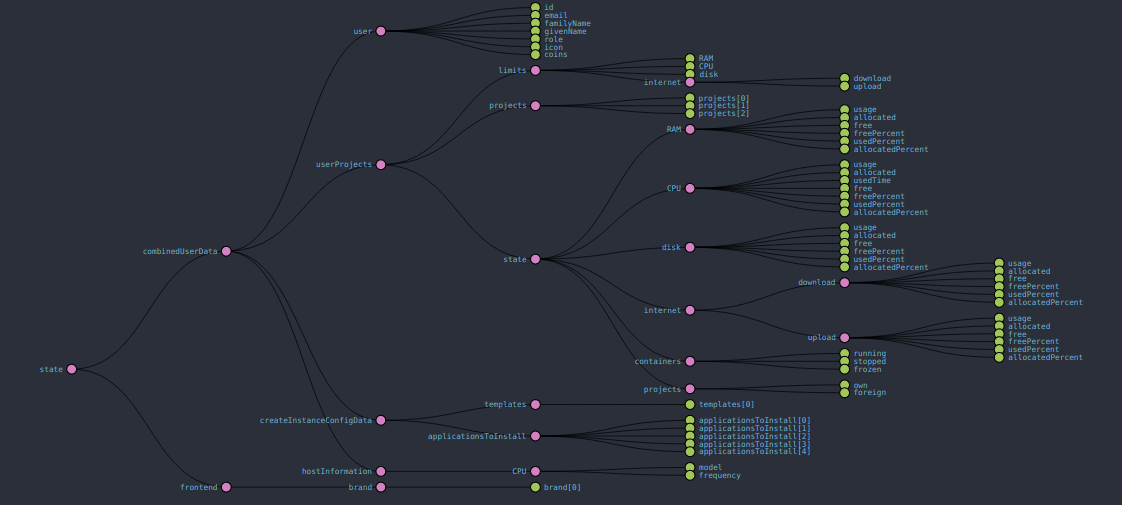
\includegraphics[height=6.9cm]{../img/Redux.png}
	\caption[Graf stavu u reduxu, vlastní tvorba, vygenerováno pomocí redux dev tools ]{Graf stavu u Reduxu}
	\label{fig:redux}
\end{figure}


Se storem je možné manipulovat pouze pomocí tzv. akcí.
Jedná se o objekty, které obsahují jméno a payload.
Tyto akce se nacházejí ve složce actions v odlišných souborech pro uživatelské akce, akce s projekty, akce s uživateli a frontendové akce.
Tyto akce mohou být tzv. dispatchnuty, čímž se dostanou k reducerům.

\begin{figure}[h]
	\dirtree{%
	.1 client.
	.2 src.
	.3 actions.
	.4 ContainerAction.js.
	.4 FrontendAction.js.
	.4 ProjectAction.js.
	.4 UserAction.js.
	}
	\caption[Struktura souborů frontendu -- actions, vlastní tvorba]{Struktura souborů frontend -- actions}
	\label{fig:frontendStructureSrc}
\end{figure}


Reducer je metoda, která na základě jména a payloadu předané akce určí, co se má stát s Redux storem.
Tento způsob změny stavu se může zdát zvláštní, každopádně zajišťuje vynikající škálovatelnost systému.
V současnosti existují v projektu dva reducery, combinedUserData reducer, který se stará o veškeré akce související se změnou dat definovaných pomocí Open API a frontend reducer, který má pouze jediný účel na frontendu.
V budoucnosti pravděpodobně nebude nutné mít více než jeden reducer, jelikož logika, kterou frontend reducer vykonává pravděpodobně bude změněna do podoby, kdy frontend reducer nebude potřeba.

Akce mohou být i asynchronní, což se např. hodí pro případ, kdy chceme poslat request na API a jakmile získáme výsledek, tak udělat se získanými daty nějakou akci - např. akce containerIdDelete() ihned zobrazí u mazaného kontejneru v tabulce kontejnerů spinner a nápis deleting.
Po smazání kontejneru se odešle na frontend odpověď a vykoná se akce smazání kontejneru z tabulky.

Jednotlivým komponentům jsou akce předávány pomocí implementace metody mapDispatchToProps, která funguje stejně jako mapStateToProps.

Hlavní účel využití Reduxu v projektu je tedy zpracování dat, které se získají z API do podoby, se kterou mohou komponenty pracovat a poskytnutí možnosti tato data měnit s okamžitými účinky na frontendu.


\section{Navigace}

O navigaci na frontendu se stará knihovna react-router.
Každá cesta na frontendu zobrazující nějakou stránku začíná prefixem daného layoutu.
V případě, že si tedy budeme chtít zobrazit hlavní panel, cesta na získání bude /user/dashboard.
Tím se vždy odliší od volání do api, které má prefix /api.

V projektu se momentálně nachází 1 + N BrowserRouterů.
Jeden v app.js, který se stará o layouty a N v rámci jednotlivých layoutů (nyní N=1).
V nich jsou vytvářeny Route objekty s adresami specifikovanými v routes.js souboru.
V něm se u každé cesty nachází také jméno dané cesty, layout, do kterého patří, navigační linky a stránka, která se má zobrazit, když uživatel zadá danou cestu.

V případě, že uživatel není přihlášen a pokusí se získat chráněný obsah, je okamžitě přesměrován na přihlašovací stránku.
Chráněným obsahem jsou přitom na frontendu s výjimkou jedné cesty úplně všechny.
V případě, že je v Redux storu proměnná combinedUserData.user null, či undefined, tak uživatel není přihlášen.
React-router ovšem neobsahuje žádný komponent ProtectedRoute, takže bylo nutné ho vytvořit.
Jedná se o klasický Route objekt kontrolující, zda je výše jmenovaná proměnná null či nikoliv.

Pro snadný pohyb po stránce byly implementovány dva druhy navigace.
Jak Navbar, tak i Sidebar jsou plně responzivní a přispůsobí se mobilnímu rozhraní, jak ve vidět na obrázcích \ref{fig:desktopRes},  \ref{fig:mobileResO} a \ref{fig:desktopRes}.

\begin{figure}[h]
	\centering
	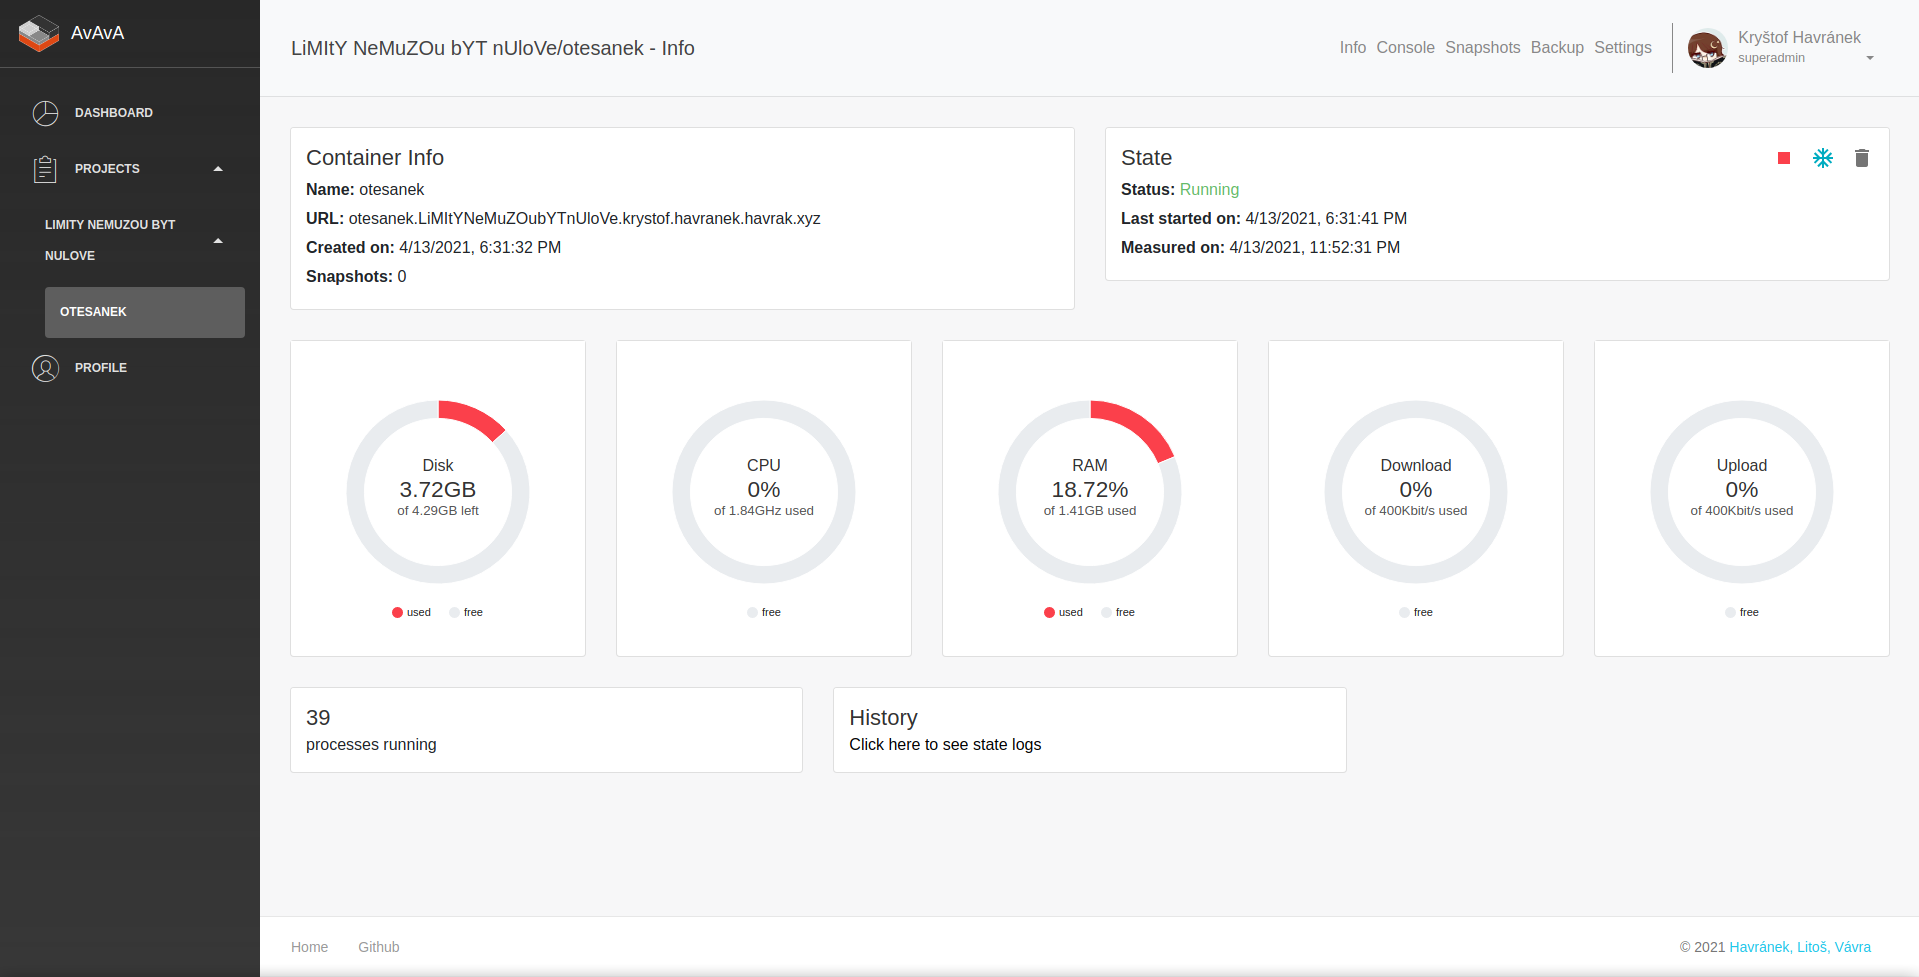
\includegraphics[height=7.8cm]{../img/navbarNonResponsive.png}
	\caption[Uživatelské rozhraní na počítači, vlastní tvorba]{Uživatelské rozhraní na počítači \linebreak}
	\label{fig:desktopRes}
\end{figure}

\begin{figure}[!htb]
	\begin{minipage}{0.48\textwidth}
		\centering
		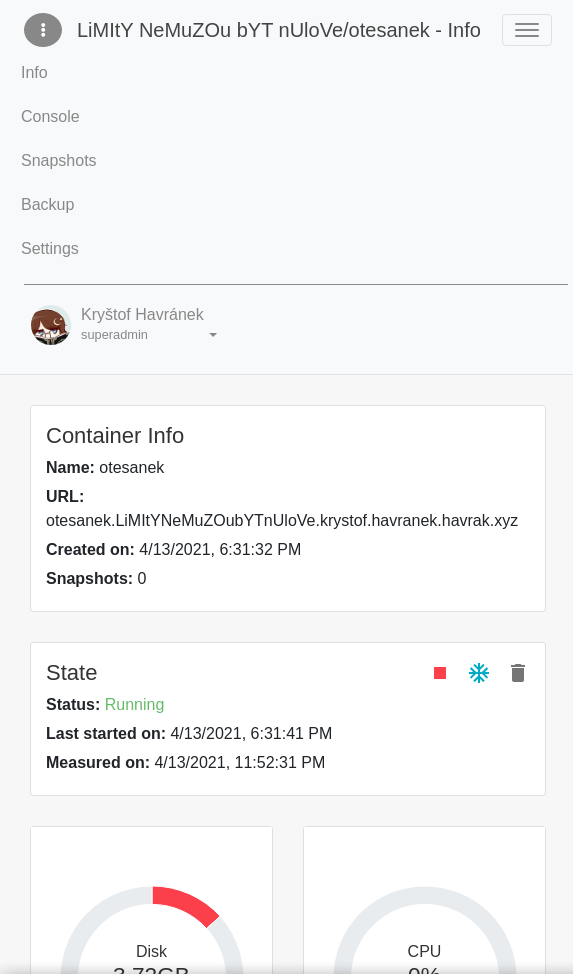
\includegraphics[height=9cm]{../img/navbarResponsiveSiderbarClosed.png}
		\caption[Responsivní interface na mobilu -- overview, vlastní tvorba]{Responsivní interface na mobilu -- overview}
		\label{fig:mobileResO}

	\end{minipage}\hfill
	\begin{minipage}{0.48\textwidth}
		\centering
		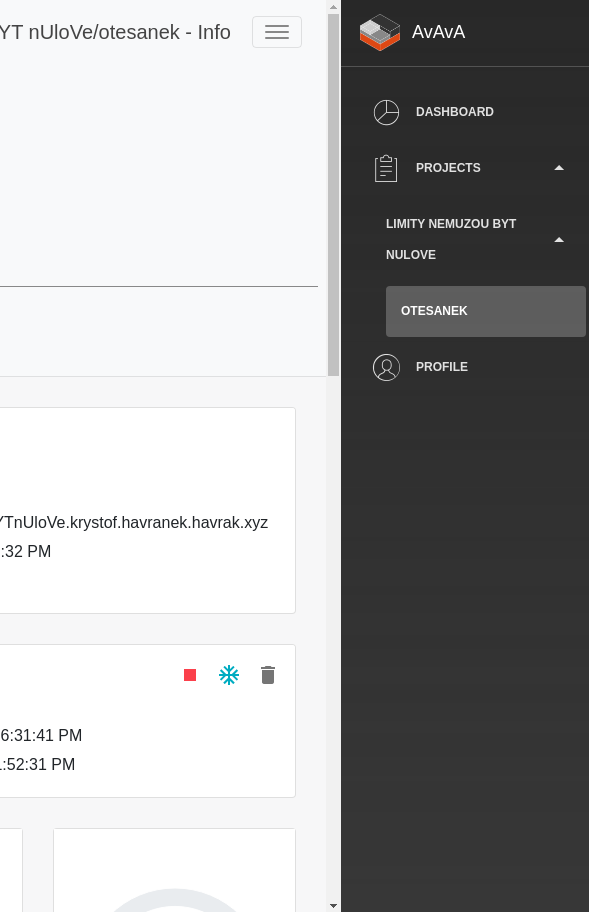
\includegraphics[height=9cm]{../img/navbarResponsiveSiderbarOpened.png}
		\caption[Responsivní interface na mobilu -- sidebar, vlastní tvorba]{Responsivní interface na mobilu -- sidebar\protect\footnotemark}
		\label{fig:mobileResS}
	\end{minipage}
\end{figure}
\footnotetext{kontent na obrazovce se posune doleva při otevření menu}

\newpage

Frontend je strukturován do 3 základních kategorií:
\begin{itemize}
	\item uživatelská - Dashboard, Projects
	\item projektová - Info, Containers, Settings
	\item kontejnerová - Info, Console, Snapshots, Backup, Settings
\end{itemize}

Sidebar - slouží převážně na přepínání mezi kategoriemi.
Dovoluje tedy jednoduše navigovat mezi projektu a jejich kontejnery.
Platí, že vždy je zvýrazněna světlým pozadím ta část sidebaru, která je momentálně zobrazovaná.
Jednotlivé projekty či kontejnery v daném projektu je možné v sidebaru rozbalit či skrýt.
Platí přitom, že nejde skrýt ta část, ve které je aktuálně zobrazený element.
Když je zadána nějaká cesta, ale daný element je zabalený, tak se rodič automaticky rozbalí.

Navbar naproti tomu má za účel navigovat převážně mezi funkcemi jedné kategorie.
Například na výše uvedeném obrázku jsou vidět funkce pro kategorie kontejner - Info, Console, Snapshots, Backup, Settings.
Zároveň se zde nachází i karta s aktuálním uživatelem, na kterou když uživatel klikne, tak mu dropdown nabídne možnost odhlásit se (viz. obrázek \ref{fig:logout}).

\begin{figure}[h]
	\centering
	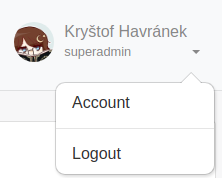
\includegraphics[height=3.8cm]{../img/logout.png}
	\caption[Odhlášení uživatele, vlastní tvorba]{Odhlášení uživatel \linebreak}
	\label{fig:logout}
\end{figure}

Vlevo se poté nachází jméno dané stránky - u kontejneru je to jméno projektu/jméno kontejneru - jméno stránky.
Zajímavostí je, že při kliknutí na jméno projektu je uživatel odkázán na Info stránku rodičovského projektu.

U obou těchto navigací platí, že jsou implementovány pomocí linků, které odkážou na nějakou cestu, jež se vykreslí za pomoci react-routeru.
Aby bylo jisté, že má uživatel vždy aktuální data, tak se při vykreslování jednotlivých cest vždy dispatchne nějaká akce, která pošle API request na server a po získání dat updatuje Redux store.
Nejprve se tedy vykreslí stará data a jakmile přijde odpověď, tak se vykreslí nová.
To dává pocit kontinuity a je to mnohem více uživatelsky přívětivé, než kdyby se čekalo na získání dat po každém kliknutí.
V budoucnosti, když se bude řešit kooperace více uživatelů se tento systém pravděpodobně změní ve prospěch nějaké formy kontrolního WebSocketu.

\section{Přehled funkcí}

Tato kapitola je věnována detailnímu popisu jednotlivých stránek a komponentů, které potřebují pro své fungování.

\subsection{Hlavní panel}

\begin{figure}[h]
	\centering
	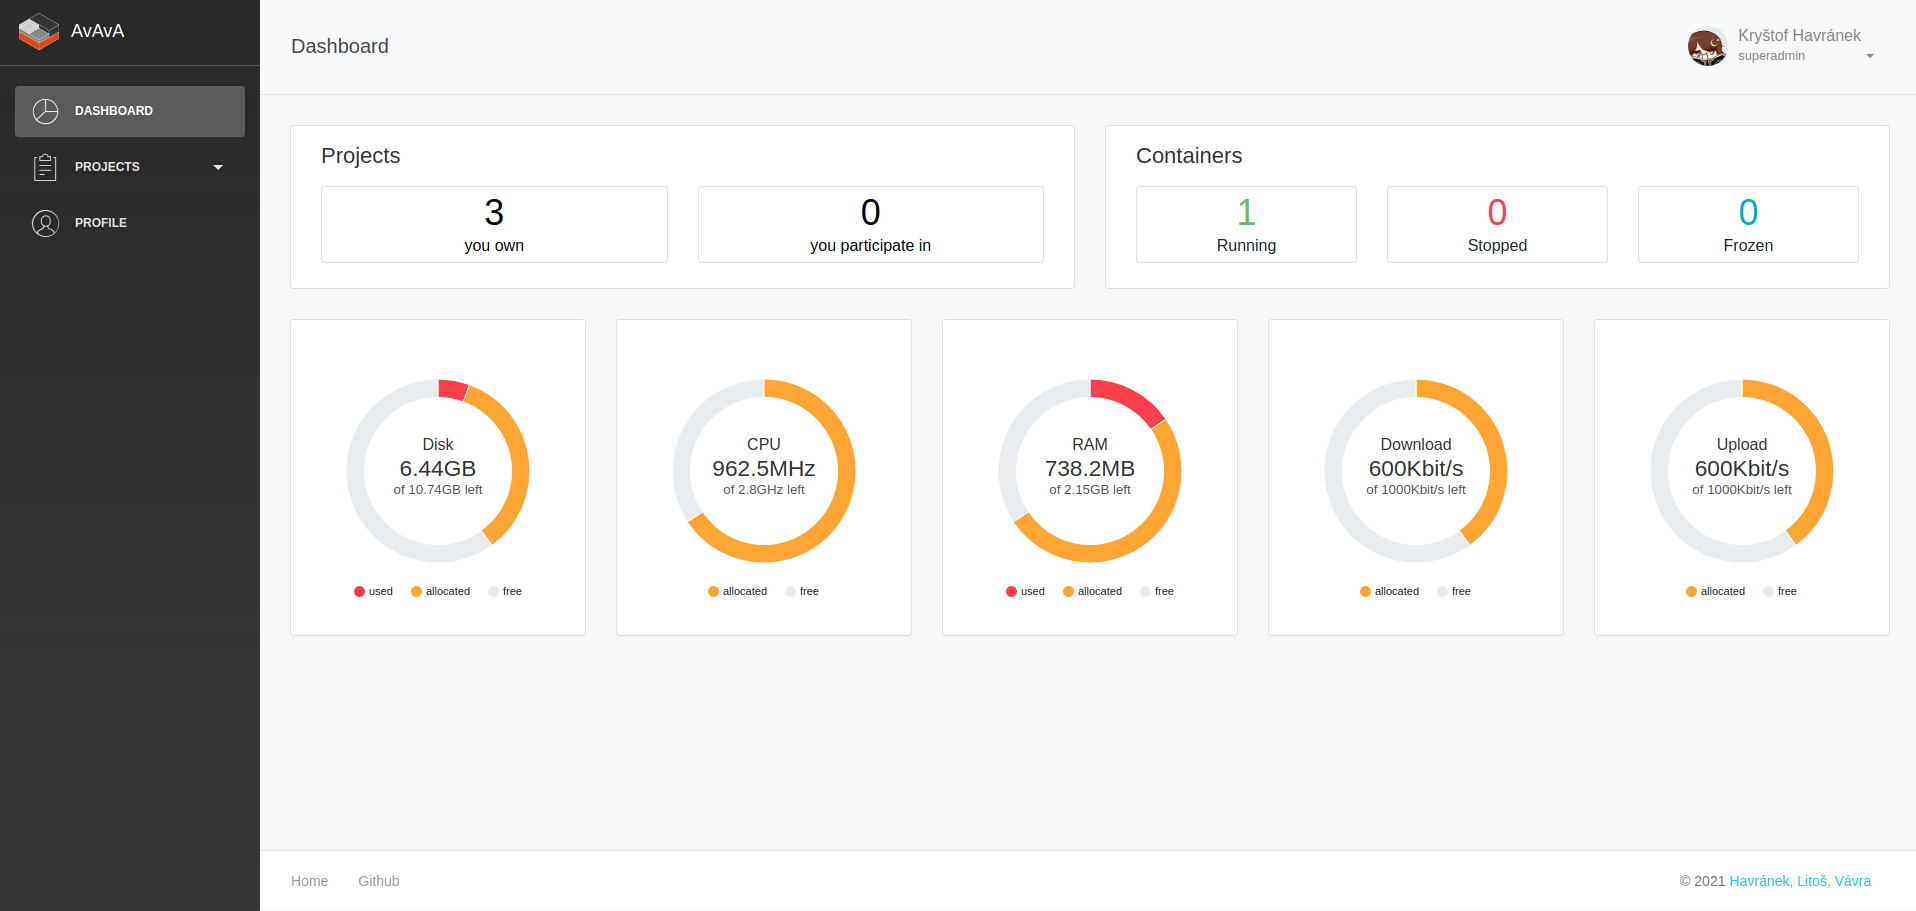
\includegraphics[height=7.3cm]{../img/dashboard.png}
	\caption[Uživatelské rozhraní na počítači, vlastní tvorba]{Uživatelské rozhraní na počítači \linebreak}
	\label{fig:desktopRes}
\end{figure}

Dashboard, neboli hlavní panel zobrazuje uživateli aktuální informace o stavu všech jeho kontejnerů a projektů.
Jedná se o první stránku, kterou po přihlášení uvidí.
Nahoře se nachází dvě karty zobrazující počet projektů, které vlastní a počet různých stavů všech jeho kontejnerů.
Nachází se zde také zobrazení počtu projektů, ve kterých se pouze účastní.
Zatím sice není implementována možnost spolupráce více uživatelů na jednom projektu, ovšem její vytvoření je plánované a jelikož Dashboard vypadá lépe s touto funkcí, tak je tato informace zobrazena již nyní.

Ve druhé řadě se nachází 5 grafů zobrazující agregovaný stav všech projektů.
Na jejich implementaci byla použita knihovna react-google-charts - pie-chart.
Červenou barvou se zobrazují zdroje, které jsou opravdu zkonzumovány jednotlivými kontejnery.
Jedná se tedy o součet usage proměnných všech kontejnerů.

Oranžově jsou poté zobrazeny zdroje, které jsou přiděleny jednotlivým projektům či přimo jednotlivým kontejnerům v případě, že samotný projekt limit nemá pro daný zdroj.
Tyto zdroje jsou zablokované a nejde je využít v jiném projektu či kontejneru než tam, kde jsou přiděleny.

Šedivě je zobrazeno volné místo, které je možné alokovat pro další projekty či kontejnery.
Toto volné místo je přitom zobrazeno uvnitř samotného grafu v adekvátních jednotkách.
Potom při umístění textu na střed grafu sehrál příspěvěk na Stack Overflowm\footnote{\bibentry{piChart}}   Dashboard zobrazuje uživatel hlavně proto, aby měl přehled o zdrojích, které může projektům alokovat, dává tedy největší smysl zobrazit právě hodnotu volného místa.
O převod ze základních jednotek se stará třída UnitsConvertor ve třídě service.
Předtím se ještě spočítat všechna potřebná data - volné zdroje, alokované zdroje, procenta, ... O to se stará třída service/StateCalculator.js, jejíž metody modifikují v reducerech stav Redux storu.
Z toho plyne, že data z Redux storu již budou mít všechna potřebná data pro zobrazení stavu k dispozici.

Komponenty grafů se nacházejí ve složce components/Cards/State.
Podobný hlavní panel jako Dashboard pro uživatelskou kategorii se nachází i v projektové a kontejnerové kategorii.
Tam ovšem fungují grafy odlišně, a tak se v této složce nacházejí ještě další dva soubory s odlišnými grafy.

\chapter{Backend}


\section{Databáze}

Sytém používá dva databázové systémy -- mySQL (mariaDB) a mongoDB.
Dle původních představ měl používat pouze mySQL.
Kvůli komplikacím s lxd, kde nejde zjistit stav zastaveného/vypnutého kontejneru, byla později zavedena mongoDB.

\subsection{mySQL}
Následující sekce se zabývá strukturou mySQL databáze a metodami, které s databází zacházejí.


\begin{figure}[h]
	\dirtree{%
	.1 src.
	.2 services.
	.3 sql.
	.4 containerSQL.js.
	.4 projectSQL.js.
	.4 templateSQL.js.
	.4 userSQL.js.
	}
	\caption[Soubory s programem týkající se mysql databáze, vlastni tvorba]{Soubory s programem týkající se mysql databáze}
	\label{fig:sqlClasses}
\end{figure}

Valnou většinu dat projekt ukládá do mySQL databáze, kde je na tento účel vytvořeno aktuálně 10 tabulek.
S databází pracují 4 soubory (viz. \ref{fig:sqlClasses}) \textit{containerSQL} zpracovává věci týkající se uživatelů, \textit{projectSQL} věci týkající se projektů, \textit{templateSQL} věci týkající se šablon a aplikací, v neposlední řadě \textit{userSQL} věci týkající se uživatele.

\subsubsection{Tabulky}

Tato sekce spěšně popíše obsah jednotlivých tabulek. A jejich vztah k ostatním. Kaskádové dependence jsou vždy stejné -- při smazání se smažou, při update se nic neděje.

\vspace{0.3cm}
\noindent
\textbf{appsToInstall} | id | name | description | icon\_path | package\_name |

Tabulka appsToInstall slouží k uložení aplikací, které je možno nainstalovat na kontejner při jeho vytváření.
Nemá žádnou vazbu na další tabulky a s jejími daty zachází třída templateSQL.
Sloupec name obsahuje jméno jaké se má zobrazit uživateli, package\_name je jméno balíčku v repositářích.

\vspace{0.3cm}
\noindent
\textbf{containers} | id | project\_id | name | url | template\_id | state | timestamp \linebreak[4] | time\_started |

Tabulka container ukládá všechny kontejnery, které spravujeme.
Obsahuje dva cizí klíče a to project\_id, které určuje do jakého projektu kontejner patří, a template\_id to určuje s jakou šablonou byl kontejner vytvořen.


\vspace{0.3cm}
\noindent
\textbf{containersResourcesLimits} | container\_id | ram | cpu | disk | upload | download |

Tabulka containersResourcesLimits ukládá limity kontejneru, stejně jako u dalších .*ResourcesLimits tabulek byla v rámci normalizačních forem oddělena od tabulky containers.
Tabulka obsahuje jeden cizí klíč, který zároveň funguje i jako primární klíč.
Veškeré limity jsou uloženy v základních jednotkách, cpu je v abstraktní jednotce herz.

\vspace{0.3cm}
\noindent
\textbf{containersResourcesLog} | container\_id | ram | cpu | number\_of\_processes | upload | download | timestamp |

Tabulka containersResourcesLog slouží k logování stavu kontejnerů.
Container\_id je cizím klíčem odkazující na kontejner, ke kterému log patří.
V aktuální verzi jsou data uložen v poli, které uložené ve sloupci s typem text.
Timestamp odkazuje na datum posledního zapsání, kdy byl zalogován předchozí stav není problém zjistit, jelikož se do tabulky zapisuje v pravidelných intervalech.

Metoda na updateování stavu (updateLogsForContainer(id, state)) si jednoduše data rozdělí dle znaku: \textbf{,}.
Do pole se přidají nové hodnoty a odebere se první prvek, nový stav se pak uloží do databáze.

Data se aktuálně do databáze uloží každých 10 minut, o což se stará cronjob (potažmo schedule) definovaný v app.js.
Aktuálně si databáze pamatuje dvanáct záznamů, takže dvě hodiny do minulosti.
Fakt, že log časový rozdíl mezi zápisy nemusí být přesně 10 minut, příliš nevadí, grafy, které se z těchto dat vykreslují jsou spíše orientační.


\vspace{0.3cm}
\noindent
\textbf{projects} | id | name | owner\_email | timestamp |

Tabulka projects si pamatuje všechny projekty, které spravuje náš systém.
Cizím klíčem je owner\_email, což je email vlastníka projektu, tedy člověka, který ho vytvořil.
Timestamp je čas vytvoření projektu.

\vspace{0.3cm}
\noindent
\textbf{projectsCoworkers} | project\_id | user\_email |

Tabulka projectsCoworkers zporstředkovává M:N vazbu mezi users a projects.
Slouží k uložení lidí, kteří jsou spolupracovnící na jednom projektu.
K datu odevzdání práce, nejsou spolupracovnící implementované, takže tabulka je aktuálně zbytečná.
Řada metoda nepočítá s existencí spolupracovníků.

\vspace{0.3cm}
\noindent
\textbf{projectsResourcesLimits} | project\_id | ram | cpu | disk | upload | download |

Tabulka projectsResourcesLimits slouží k uložení limitů projektu.
Nerozdíl od containersResourcesLimits můžou zde mít limity hodnotu null.
V takovém případě je kontejnerům dostupný vešerý volný prostor, který uživatel má.

\vspace{0.3cm}
\noindent
\textbf{templates} | code | id | profile\_name | image\_name | version | profile\_description | image\_description | profile\_path | min\_disk\_size |

Tabulka templates slouží k uložení šablon, lde kterých se má vytvořit kontejner.
Šablona je koncept, který se nenachází přímo v lxd, ale integruje dvě věci -- profily a image.
Image je distribuce jaká se na systém má nainstalovat.
Profile je koncept z lxd, který obsahuje konfiguraci kontejneru.
Eventuálně by měl uživatel možnost vytvářet si vlastní profily, které by obsahovali například konfiguraci networků.

\vspace{0.3cm}
\noindent
\textbf{users} | id | email | given\_name | family\_name | icon | role | coins |

Tabulka users slouží k uložení uživatelů.
Svoje data dostává z dat, které zasílá googleAuth 2.0.
Sloupce role a coins aktuálně nemají význam, role bude dělit uživatele mezi standardního uživatel, admina a superadmin.
Admin a superadmin by měli právo zasahovat do kontejnerů jiných uživatelů.
Coins měl být sloupec sloužící u ekonomiky systému, k její implementaci však nedošlo.


\vspace{0.3cm}
\noindent
\textbf{usersResourcesLimits} | user\_id | ram | cpu | disk | upload | download |

Tabulka usersResourcesLimits ukládá limity uživatelů.
Aktuálně má uživatel k dispozici 2.8 GHz\footnote{server kde byl program vyvíjen měl 2 jádra o 2.8 GHz, jedná se tak o polovinu výkonu}, 2 GB ram, 8GB volného místa na disku, a download a upload 800kb/s.

\subsection{mongoDB}


\section{LXD}

\section{Networking}

Následující sekce se zabývá networkingem kontejnerů a proxy, které umožňuje přístup na ně z venčí.

\subsection{Konfigurace networků}

Pomineme li loopback (standardní \textit{lo}), tak každý kontejner má v aktuální verzi právě jeden networkový interface.
Tím je \textit{eth0}, který je na hostovi napojen na bridge \textit{lxdbr0}.
Přes něj mají kontejnery přístup na internet.
Zároveň jsou všechny na stejné síti (prostřednictvím \textit{lxdbr0})

Jelikož jsou veškeré kontejnery na stejné síti, tak mezi sebou mohou komunikovat.
Lxd pro tento účel samo nastavuje jejich interní doménu, ta je ve tvaru \textit{c\{id\}.lxd}.
Pochopitelně však nejsou dostupné z internetu, doména je pouze interní a veřejnou ip adresu nemají.
Aby bylo možno na kontejner přistupovat bylo nutné nastavit proxy, které mu databáze bude přeposílat.

Nutno podotknout, že i traffic mezi kontejnery je aktuálně omezen limitem.
V budoucno se tedy nabízí možnost implementovat možnost vytvářet další bridge a kontejnery si propojovat.
Ty by se mohly ukládat do profilů, uživatel by si tak rovnou mohl vytvořit kontejnerů izolovaný od ostatních.

Fakt, že kontejnery jsou na stejné síti není rizikové ani problematické.
Standartě se nemůžou nijak ovlivňovat.

\subsection{Proxy}

Pro proxy využívá projekt volně dostupnou haproxy, jejíž instance běží ve stejnojmenném kontejneru.
Hostovací stroj totiž standardně nemůže přistupovat na kontejnery prostřednictvím .lxd domény.
Bylo by možné sice mít proxy na hostovi serveru, ale z bezpečnostních důvodů tak nebylo učiněno.

Do kontejneru haproxy je aktuálně přesměrována traffic ze čtyř portů -- 80, 443, 2222 a 3000.
Port 80 pochopitelně slouží na webové stránky pomocí protokolu http.
443 je pro https, proxy má nastavený ssl certifikát.
Ten stačí jeden pro celý systém, musí se však jednat o certifikát typu wildcard\footnote{certifikát, který zahrnuje i subdomény}.
Systém byl testován na standardním certifikátu, čily připojení sice bylo zabezpečené, ale prohlížeč hlásil podezření z fishningu, jelikož se doména a doména na certifikátu neschodovali.
Port 2222 slouží na připojení přes ssh, port 22 používá hostovací stroj a z pochopitelných důvodů není přesměrován do proxy.
Port 3000 je dostupný pro REST API aplikací, které na serveru budou běžet.

Kotejnerům je automaticky přirazena doména v následujícím tvaru \textit{\{jméno kotejneru\}.\{jméno projekty\}.\{část emailu uživatel, před @\}.\{doména serveru\}}.
Například kontejner pojmenovaný \textit{rumburak} v projektu \textit{web} uživatele \textit{belzebub@email.com} na serveru s doménou \textit{avava.cz} bude mít doménu {rumburak.web.belzebub.avava.cz}.
Mezery ve jméně kontejneru, či projektu se domény odstraní.
Pokud by měl nový kontejner stejné jméno, jako jiný systém vyhodí výjimku.
Tak je zaručena unikátnost domén, u mailu není takový problém nutno řešit, jelikož se jedná o školní emaily, které jsou vždy unikátní.

Bohužel je možno elegantně forwardovat pouze http protokol.
Většina TCP protokolů totiž neoperuje s SNI a řídí se pouze doménu.
Z packetu tak nejde zjistit na jakou doménu se uživatel snaží dostat a tedy jakému kontejneru mý být protokol přiřazen.
To by se týkalo i ssh, příkaz ssh však podporuje nastavit pomocí flagu -o ProxyCommand (viz. \ref{fig:sshcom}), packety poté sni v hlavičce mají a je možno poznat jakému kontejneru patří.
\begin{figure}[h]
\begin{lstlisting}[breaklines]
ssh -o ProxyCommand="openssl s_client -connect $SERVERURL:2222 -servername $CONTAINERURL" blank -l $USERNAME
\end{lstlisting}
\caption[Příkaz k připojení na server, vlastní tvorba]{Příkaz k připojení na server\protect\footnotemark}
\label{fig:sshcom}
\end{figure}
\footnotetext{\$SERVERURL je url serveru kde běží kontejnerizační systém, \$CONTAINERURL je url kontejneru, \$USERNAME je jméno uživatel, argument dummy je ignorován, je však potřeba}

Porty jako 8443 aktuálně forwardovány nejsou, pokud uživatel potřebuje přistupovat do datáze běžící na kontejneru je možno použít ssh local port forwarding.
Tento princip je i bezpečnější.

Konfigurační soubor HAProxy je generován v containerSQL.js.
Po jeho vygenerování se prostřednictvím lxd.postFileToInstance pošle nová konfigurace to HAProxy kontejneru.
Restartování proxy je téměř instantní operace i s velkým konfiguračním souborem obsahujícím desítky kontejnerů.
Downtime je tak minimální.
Podoba konfigurace byla realizována za pomocí dokumentace HAProxy\footnote{\bibentry{HaproxyDocs}}.
Aktuálně má formát konfiguračního souboru jisté rezervy, specificky co se týče jeho délky.
Je však o trochu rychlejší než, kdyby byly použity pokročilé metody mapování, které HAProxy podporuje.


% \chapter{Obrázky systému}
% \begin{figure}[h]
% 	\centering
% 		\includegraphics[height=8cm]{../img/dataatad.jpg}
% 		\caption[Obrazovka při běhu programu]{
% 		Obrazovka při běhu programu
% 	}
% \end{figure}

% \begin{figure}[h]
% 	\centering
% 		\includegraphics[height=8cm]{../img/sys.jpg}
% 		\caption[Obrazovka s 2 moduly M5Stack]{
% 		Obrazovka s 2 moduly M5Stack
% 	}
% \end{figure}

\chapter*{}
\pagenumbering{roman}
\setcounter{page}{6}
\chapter*{Závěr}
\addcontentsline{toc}{chapter}{Závěr}

Ačkoliv jsme původně měli vyšší nároky na náš projekt, které se kvůli špatnému vyhodnocení obtížnosti způsobené malými předchozími zkušenostmi členů týmu s full stack vývojem a špatným dokumentacím závislostí práce, zatím nepodařilo splnit, hodnotíme práci jako úspěch. Kritické části práce fungují, uživatel si může jednoduše vytvořit kontejner. V něm deploynout svojí aplikaci, a vyzkoušet si tak, jaké to je být adminem na linuxovém serveru. Byl tedy vytvořen funkční systém pro vytváření a správu kontejnerů, který může být po menších úpravách nasazen na školní server.

V budoucnosti bychom rádi dokončili všechny funkce, které jsme původně chtěli implementovat. V aktuálním systému jsou jimi práce se Snapshoty kontejnerů, import záloh, zobrazení historie stavů kontejnerů a projektů a systém na dokoupení uživatelských limitů. Je také nutné otestovat, při jakých limitech je možné vytvářet dobré podmínky pro studentské aplikace, aby se maximalizovala efektivita rozdělování zdrojů.

Systém bychom ovšem chtěli rozšířit ještě víc tím, že bychom přidali administrátorský účet a super-administrátorský účet na správu samotné aplikace. Nakonec máme ještě v plánu vytvořit real-time systém pro kooperaci uživatelů na jednom projektu. S již vylepšenou prací bychom se rádi příští zúčastnili soutěže SOČ.




%%% Seznam použité literatury (bibliografie)
%%%
%%% Pro vytváření bibliografie používáme bibTeX. Ten zpracovává
%%% citace v textu (např. makro \cite{...}) a vyhledává k nim literaturu
%%% v souboru literatura.bib.
%%%
%%% Příkaz \bibliographystyle určuje, jakým stylem budou citovány odkazy
%%% v textu. V závorce je název zvoleného souboru .bst. Styly plainnat
%%% a unsrt jsou standardní součástí latexových distribucí. Styl czplainnat
%%% je dodáván s touto šablonou a bibTeX ho hledá v aktuálním adresáři.

\bibliographystyle{czplainnat}   %% Autor (rok) s českými spojkami
%\bibliographystyle{plainnat}    %% Autor (rok) s anglickými spojkami
%\bibliographystyle{unsrt}       %% [číslo]


\renewcommand{\bibname}{Seznam použité literatury}

%%% Vytvoření seznamu literatury. Pozor, pokud jste necitovali ani jednu
%%% položku, seznam se automaticky vynechá.

\bibliography{literatura}

%%% Kdybyste chtěli bibliografii vytvářet ručně (bez bibTeXu), lze to udělat
%%% následovně. V takovém případě se řiďte normou ISO 690 a zvyklostmi v oboru.

% \begin{thebibliography}{99}
%
% \bibitem{lamport94}
%   {\sc Lamport,} Leslie.
%   \emph{\LaTeX: A Document Preparation System}.
%   2. vydání.
%   Massachusetts: Addison Wesley, 1994.
%   ISBN 0-201-52983-1.
%
% \end{thebibliography}


\listoffigures
\openright
\end{document}
